\documentclass[a4paper,12pt]{article}
\usepackage{graphicx}
\usepackage{lipsum} 
\usepackage{ragged2e}
\usepackage{hyperref}
\usepackage{parskip} 
\usepackage{listings}
\lstset{basicstyle=\ttfamily,breaklines=true}

\begin{document}

\begin{titlepage}
      \begingroup
      \centering
      
\includegraphics[width=0.5\textwidth]{sapienza.png}\par\vspace{1cm}

      {\bfseries\large Data Management Project \par}\vspace{0.5cm}

      {\bfseries\LARGE Mamo Art Gallery \par}\vspace{1cm}

      {\small Faculty of Information Engineering, Computer Science and Statistics
            \par}\vspace{0.1cm}

      {\small
            M.Sc. Engineering in Computer Science
            \par}\vspace{10cm}

      \endgroup

      {\textbf{\small
                  Presented by: \\
                  Gloria Marinelli, 2054014 \\
                  Mario Morra, 2156770}}\vfill

\end{titlepage}

\tableofcontents
\newpage

\section{Introduction}
\justify
The idea is a web-based application which serves as an online marketplace for the search and purchase of artworks created by a number of different artists. Potential users are afforded the opportunity to explore a variety of paintings prior to making a purchase.

The application's architectural framework consists of the following components:

\begin{itemize}
      \item A \textbf{database}, managed by MongoDB.
      \item A \textbf{backend}, constructed using Python with the Flask web framework.
      \item A \textbf{frontend}, developed using the ReactJS framework.
\end{itemize}

The entire application is based on two datasets: the \href{https://www.kaggle.com/datasets/isaienkov/edvard-munch-paintings}{Edvard Munch Paintings } dataset and the \href{https://www.kaggle.com/datasets/momanyc/museum-collection?select=artworks.csv}{Museum of Modern Art (MoMA) Collection} dataset.

The web application is structured as follows:

\begin{itemize}
      \item The \textbf{login page}
      \item the \textbf{sign up page}

      \item The \textbf{homepage}: displays all available paintings at MaMo Art gallery. Selecting a painting will display a summary of relevant information about the artwork, including the title, name, date, medium, dimensions, acquisition date, and other pertinent details. Furthermore, users have the option to purchase the selected artwork directly from this page, which will then be added to their list of orders.

      \item The \textbf{orders page}: displays all orders placed by the user, including the Order ID, the Artwork ID and the date of the order.

      \item The \textbf{artists page}:  displays all artists associated with MaMo Art Gallery. Clicking on an artist displays their biography (nationality, gender, birth year, death year) and the list of their relative paintings.

\end{itemize}

\newpage
\section{Dataset Description}
\justify

The application is built upon two datasets: the \href{https://www.kaggle.com/datasets/isaienkov/edvard-munch-paintings}{Edvard Munch Paintings } dataset and the \href{https://www.kaggle.com/datasets/momanyc/museum-collection?select=artworks.csv}{Museum of Modern Art (MoMA) Collection} dataset.


The \textbf{first} dataset includes all known paintings created by the Norwegian artist Edvard Munch. This dataset consists of 1,789 entries, each providing metadata related to Munch's paintings. The columns in the dataset are as follows:


\begin{itemize}
      \item \textbf{number}: index number of the painting
      \item \textbf{name}: title of the painting
      \item \textbf{year}: year of creation
      \item \textbf{location}: current location of the painting
      \item \textbf{status}: indicates whether the painting is lost (no image exists)
      \item \textbf{technique}: technique used in creating the painting
      \item \textbf{size}: original dimensions of the painting
      \item \textbf{filename}: image file name in the dataset
\end{itemize}


The \textbf{second} dataset is the MoMA Collection, which includes comprehensive records of artworks and artists represented in the museum. This dataset is divided into two CSV files: one containing artworks, with 218,000 records, and the other containing artists, with 67,700 records.
\begin{itemize}
      \item \texttt{artworks.csv} contains the following columns:
            \begin{itemize}
                  \item \textbf{artwork id}: unique identifier for the artwork
                  \item \textbf{title}: title of the artwork
                  \item \textbf{artist id}: identifier for the artist
                  \item \textbf{name}: name of the artist
                  \item \textbf{date}: date of the artwork
                  \item \textbf{medium}: material or technique used
                  \item \textbf{dimensions}: physical dimensions of the artwork
                  \item \textbf{acquisition date}: date when the artwork was acquired by moma
                  \item \textbf{credit}: source of acquisition
                  \item \textbf{catalogue}: catalogue information
                  \item \textbf{department}: department within moma responsible for the artwork
                  \item \textbf{classification}: artwork classification
                  \item \textbf{object number}: unique identifier for the object in the museum’s system
                  \item \textbf{diameter (cm)}, \textbf{circumference (cm)}, \textbf{height (cm)}, \textbf{length (cm)}, \textbf{width (cm)}, \textbf{depth (cm)}, \textbf{weight (kg)}, \textbf{duration (s)}: physical measurements of the artwork, where applicable

            \end{itemize}

      \item \texttt{artists.csv} contains the following columns:
            \begin{itemize}
                  \item \textbf{artist id}: unique identifier for the artist
                  \item \textbf{name}: name of the artist
                  \item \textbf{nationality}: nationality of the artist
                  \item \textbf{gender}: gender of the artist
                  \item \textbf{birth year}: year of birth
                  \item \textbf{death year}: year of death (if applicable)
            \end{itemize}
\end{itemize}

\newpage
\section{Database: MongoDB}
\justify

\textbf{MongoDB} is an open-source database designed for flexibility and scalability. It stores data in documents, making it easy to handle complex data. MongoDB can handle large amounts of unstructured data and can be scaled horizontally. MongoDB also offers features like replication, high availability, and indexing for better performance. It can be scaled horizontally through sharding, which distributes data across multiple servers for better performance and reliability.


\subsection{Why use MongoDB?}
\justify
\textbf{MongoDB} is a good choice for the \textbf{MaMo Art Gallery} web app. The datasets contain different types of data, including paintings, artists, dimensions and acquisition history. MongoDB's \textbf{document-oriented approach} is ideal for this application because it can combine different datasets without any predefined relationships. MongoDB also supports quick searches and indexing, which is important for the marketplace. Furthermore, users can browse, order and view order histories in real time.

\subsection{Analysis and management of data}
\justify

The \texttt{database.py} script loads painting and artist data from CSV files into a MongoDB database. It cleans the data, removes duplicate painting titles, and inserts the records into a \textit{paintings} collection. It also creates separate collections for each artist to avoid duplicates, with Edvard Munch's paintings stored in both general and specific collections. Finally, it loads the artist data into an \textit{artists} collection, resulting in the MaMo-Art database containing \textit{paintings}, \textit{artists}, and individual collections for each artist.

\textbf{CSV file reading and parsing}

The data pertaining to paintings and artists is extracted from CSV files $\left(\texttt{paintings.csv}, \texttt{edvard\_munch.csv}, \texttt{artists.csv}\right)$ using the \textit{CSV} library. These files contain information on paintings and artists, and each row is processed in turn, with any unnecessary data removed.

\textbf{Text cleaning}

The CSV files are cleaned by removing unnecessary spaces and commas to ensure data consistency before insertion and normalization. Furthermore, any special characters in collection names are removed, such as dots at the end of artist names, to prevent any potential naming issues when creating MongoDB collections.

To avoid repetition of entries for paintings and artists within the database, the titles of paintings are stored in a set $\left(\texttt{paintings\_titles}\right)$, thus simplifying the identification of duplicates during data processing.

\textbf{Inserting data into MongoDB}

Once the data has been cleaned and deduplicated, it is inserted into MongoDB collections. Each painting or artist is represented as a document in the database. This is achieved using the \textit{insert\_one} method, which allows for the addition of each record individually.

\textbf{Managing MongoDB collections for specific artists}

Paintings are inserted not only into the aggregate collection of \textit{paintings}, but also into distinct collections for specific artists using the \texttt{update\_one} method. For instance, Edvard Munch's artworks are included in both the main collection and a dedicated collection for the artist, \textit{Edvard Munch}.

\textbf{Handling collections}

To prevent the replication of paintings during updates, the \texttt{update\_one} method with the \texttt{upsert=True} parameter guarantees the insertion of new paintings into the collection if they do not already exist. This is employed when associating paintings with specific artists within their respective collections.

\textbf{Handling duplicate checks for Edvard Munch}

A specific check is carried out to determine whether a painting by Edvard Munch is already present in one of the collections. In the case that a duplicate is identified, the insertion is cancelled.


\subsection{Sharding}
\justify

The technique of \textbf{sharding} in MongoDB is employed to distribute data across multiple servers, thereby enhancing the performance, scalability, and reliability of large-scale databases. When a dataset reaches the limits of a single server's capacity, sharding enables horizontal scaling through the partitioning of data into smaller units, called \textbf{shards}, which are then distributed across multiple servers. Each shard contains a portion of the complete dataset.

In the context of the \textbf{MaMo Art Gallery}, the implementation of sharding could prove particularly beneficial as the size of the dataset (including the large number of paintings, artist details, and user orders) increases over time.

\subsubsection{Configuring sharding}
This section explains how to set up sharding in MongoDB. It involves creating multiple shards, setting up configuration servers, starting replica sets, and enabling sharding for a specific database. Here’s an explanation of each step.

\begin{itemize}
      \item \textbf{Creating directories for shards and config servers}

            \begin{lstlisting}
    mkdir C:\data\shard1
    mkdir C:\data\shard2
    mkdir C:\data\shard3
    mkdir C:\data\config1
    mkdir C:\data\config2
    mkdir C:\data\config3
    \end{lstlisting}

            Directories are created to store data for shards and config servers. Shards store parts of the database, while config servers manage the information for the sharded cluster.

      \item \textbf{Starting MongoDB instances for each shard}

            \begin{lstlisting}
    .\mongod --shardsvr --replSet shard1 --port 27001 --dbpath C:\data\shard1 
    .\mongod --shardsvr --replSet shard2 --port 27002 --dbpath C:\data\shard2 
    .\mongod --shardsvr --replSet shard3 --port 27003 --dbpath C:\data\shard3
    \end{lstlisting}

            Three MongoDB instances are started on different ports (\textbf{27001, 27002} and \textbf{27003}), each representing a shard in the cluster. The \texttt{--replSet} option names each replica set (\textbf{shard1, shard2, shard3}).


      \item \textbf{Initiating replica sets for the shards}

            \begin{lstlisting}
    .\mongosh --port 27001
    rs.initiate()

    .\mongosh --port 27002
    rs.initiate()

    .\mongosh --port 27003
    rs.initiate()
    \end{lstlisting}

            Each shard is configured as a replica set, ensuring that data is copied for safety and high availability.

      \item \textbf{Starting and configuring config servers}

            \begin{lstlisting}
    .\mongod --configsvr --replSet configReplSet --port 27020 --dbpath C:\data\config1 
    .\mongod --configsvr --replSet configReplSet --port 27021 --dbpath C:\data\config2
    .\mongod --configsvr --replSet configReplSet --port 27022 --dbpath C:\data\config3
    \end{lstlisting}

            Three MongoDB instances store metadata for the sharded cluster. The \texttt{--configsvr} flag designates these instances as config servers. They are part of a replica set called \texttt{configReplSet} to ensure high availability.

      \item \textbf{Initiating the config server replica set}

            \begin{lstlisting}
    .\mongosh --port 27020
    rs.initiate({
       _id: "configReplSet",
       configsvr: true,
       members: [
          { _id: 0, host: "localhost:27020" },
          { _id: 1, host: "localhost:27021" },
          { _id: 2, host: "localhost:27022" }
       ]
    })
    \end{lstlisting}

            The config server replica set is initiated by specifying its members on ports \textbf{27020, 27021}, and \textbf{27022}.

      \item \textbf{Starting the \texttt{mongos} router}

            \begin{lstlisting}
    .\mongos --configdb configReplSet/localhost:27020,localhost:27021,localhost:27022 --port 27018
    \end{lstlisting}

            A \texttt{mongos} instance is started on port \textbf{27018}. The \texttt{mongos} routes queries to the appropriate shard and connects to the config servers to get cluster information.

      \item \textbf{Adding shards to the cluster}

            \begin{lstlisting}
    .\mongosh --port 27018

    sh.addShard("shard1/localhost:27001")
    sh.addShard("shard2/localhost:27002")
    sh.addShard("shard3/localhost:27003")
    \end{lstlisting}

            Each shard is added to the cluster using the \texttt{addShard} command. The system now recognizes \textbf{shards 1, 2}, and \textbf{3} as part of the sharded database.

      \item \textbf{Enabling sharding for the database}

            \begin{lstlisting}
    sh.enableSharding("MaMo-Art")
    \end{lstlisting}

            Sharding is enabled for the \texttt{MaMo-Art} database, allowing the distribution of collections across the shards.

      \item \textbf{Sharding the paintings collection}

            \begin{lstlisting}
    use MaMo-Art
    sh.shardCollection("MaMo-Art.paintings", { "_id": "hashed" })
    \end{lstlisting}

            The \texttt{MaMo-Art} database is sharded based on the \texttt{\_id} field. A hashed sharding key ensures that data is distributed evenly across shards.

      \item \textbf{Checking sharding status and starting the balancer}

            \begin{lstlisting}
    sh.status()
    sh.startBalancer()
    \end{lstlisting}

            The status of the sharded cluster is checked using \texttt{sh.status()}, and the balancer is started. The balancer helps distribute data across shards to prevent any one shard from becoming overloaded.
\end{itemize}

\newpage
\section{API Development: Flask}
\justify

The \texttt{server.py} file defines a \textbf{Flask-based} web application programming interface (\textbf{API}) that interacts with a MongoDB database for the purpose of managing paintings and user data. Additionally, indexes are employed on relevant fields to enhance query performance and responses are consistently formatted in \textbf{JSON}.


\subsection{API Endpoints} \justify The \textbf{API} has many endpoints that interact with the database. These include user authentication, managing painting data, searching, filtering, and handling cart operations. The following is a detailed overview of the available API endpoints, their purpose and how they interact with the database.


\begin{itemize}

      \item \textbf{/register} (POST): it is used to register new users. It accepts a JSON body containing the \textbf{username, name}, and \textbf{password} of the user, and stores this information in the \textit{user} collection. Before storing the user, the system checks if the username already exists to prevent duplicate entries.

      \item \textbf{/login} (POST): handles user login by checking that the \textbf{username} and \textbf{password} match the credentials stored in the \textit{user} collection. If they match, a successful login response is returned, otherwise an error message.

      \item \textbf{/getPaintings} (GET): returns all paintings from the \textit{paintings} collection without applying any filters or sorting mechanisms.

      \item \textbf{/getDepartments} (GET): returns a unique list of all the departments from the \textit{paintings} collection, allowing the clients to obtain department names without retrieving all data.


      \item \textbf{/getPaintingsFilter} (GET): returns paintings from the \textit{paintings} collection, based on filters such as \textbf{title, department} and \textbf{name} (at least one parameter is required, otherwise an error is returned). It uses a \textbf{compound index} on these fields to improve query performance.

      \item \textbf{/getPaintingsDetails} (GET): returns a specific painting from the \textit{paintings} collection based on the provided \textbf{id} parameter. It utilises an \textbf{index} on the \textbf{id} field to enhance lookup speed.

      \item \textbf{/addtocart} (GET): adds an item to the user's cart. The request takes three parameters: an \textbf{order ID}, a \textbf{username}, and an \textbf{artwork ID}. These are inserted into the \textit{orders} collection with a timestamp.

      \item \textbf{/getArtists} (GET): returns a list of all collections that have been named in accordance with the artist's name and that are currently stored in the database. It excludes collections of  \textit{users, paintings, orders} and \textit{artists}. This lists available artists without returning unnecessary collections.

      \item \textbf{/getPaintingsArtistCollection} (GET): returns all paintings from a specific \textit{artist}'s collection. The \textbf{name of the artist} is provided as a parameter, and the paintings are retrieved from the corresponding collection.

      \item \textbf{/getBio} (GET): fetches the biography of a specific artist from the \textit{artist}'s collection. The \textbf{name of the artist} is provided as a query parameter, and if a match is found, the artist's biography is returned.

      \item \textbf{/getUserOrders} (GET): returns all orders that are associated with a specific username. The endpoint employs an \textbf{index} on the \textbf{username} field to enhance the efficiency of queries, returning a list of \textbf{order IDs, artwork IDs,} and \textbf{timestamps} in descending order.

\end{itemize}

\section{Performance Analysis}
In order to balance the measurements and comparisons, the analysis was always performed on the same sample.

\subsection{getPaintingsTitle vs getPaintingsTitleByIndex}


\textbf{getPaintingsTitle}: The proposed solution does not use indexes and instead relies on the following query:
\begin{lstlisting}[language=Python]
query = {"title": {"$regex": title, "$options": "i"}}
\end{lstlisting}
This query uses a regular expression to perform a case-insensitive search on the \textbf{title}. However, the use of regular expressions, especially without indexing, results in a \textbf{full collection scan}, which is inefficient for large datasets, particularly for fields such as \textbf{title} that have high cardinality. Therefore, this approach has a considerable impact on performance that can be potentially slow and inefficient.

\begin{figure}[h]
      \centering
      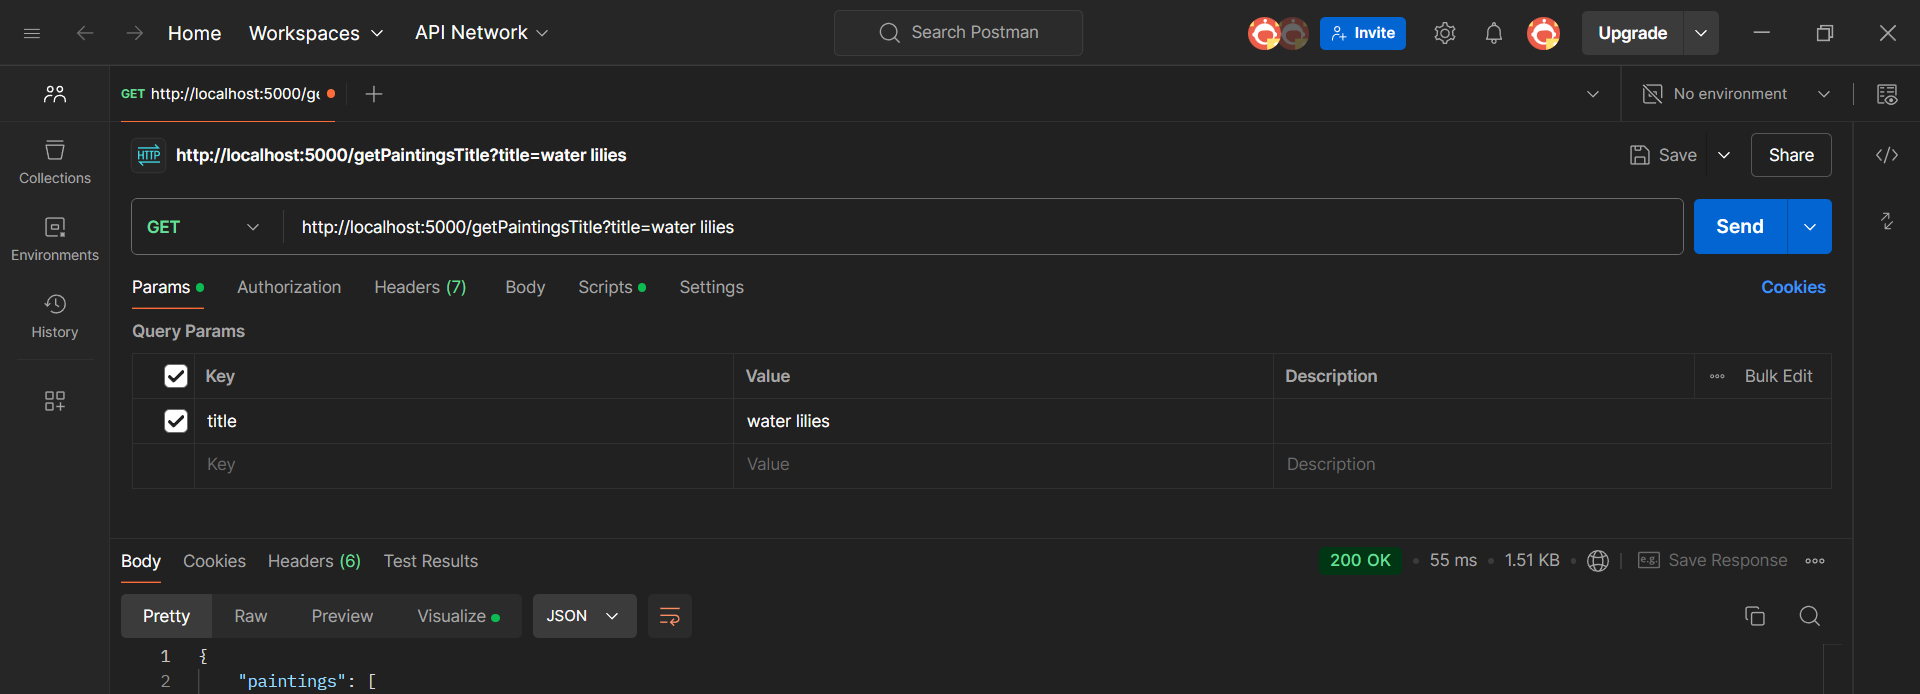
\includegraphics[width=1\textwidth]{images/getPaintingsTitleS.png}
      \caption{getPaintingsTitle}

\end{figure}

\textbf{getPaintingsTitleByIndex}: On the other hand, this endpoint is designed to enhance query performance by creating an \textbf{index} on the \textbf{title} field:
\begin{lstlisting}[language=Python]
paintings_coll.create_index([("title", ASCENDING)], name="title_index")
\end{lstlisting}
The use of the index rapidly identifies matching documents, rather than conducting a \textbf{full scan} of the entire collection. Indeed, this approach \textbf{reduces the search space}, enhancing the efficiency of the query. Furthermore, the index guarantees that the query is \textbf{sorted} in \textbf{ascending order} based on the \textbf{title}, as follows:
\begin{lstlisting}[language=Python]
paintings = list(paintings_coll.find(query).sort("title", ASCENDING))
\end{lstlisting}

\begin{figure}[h]
      \centering
      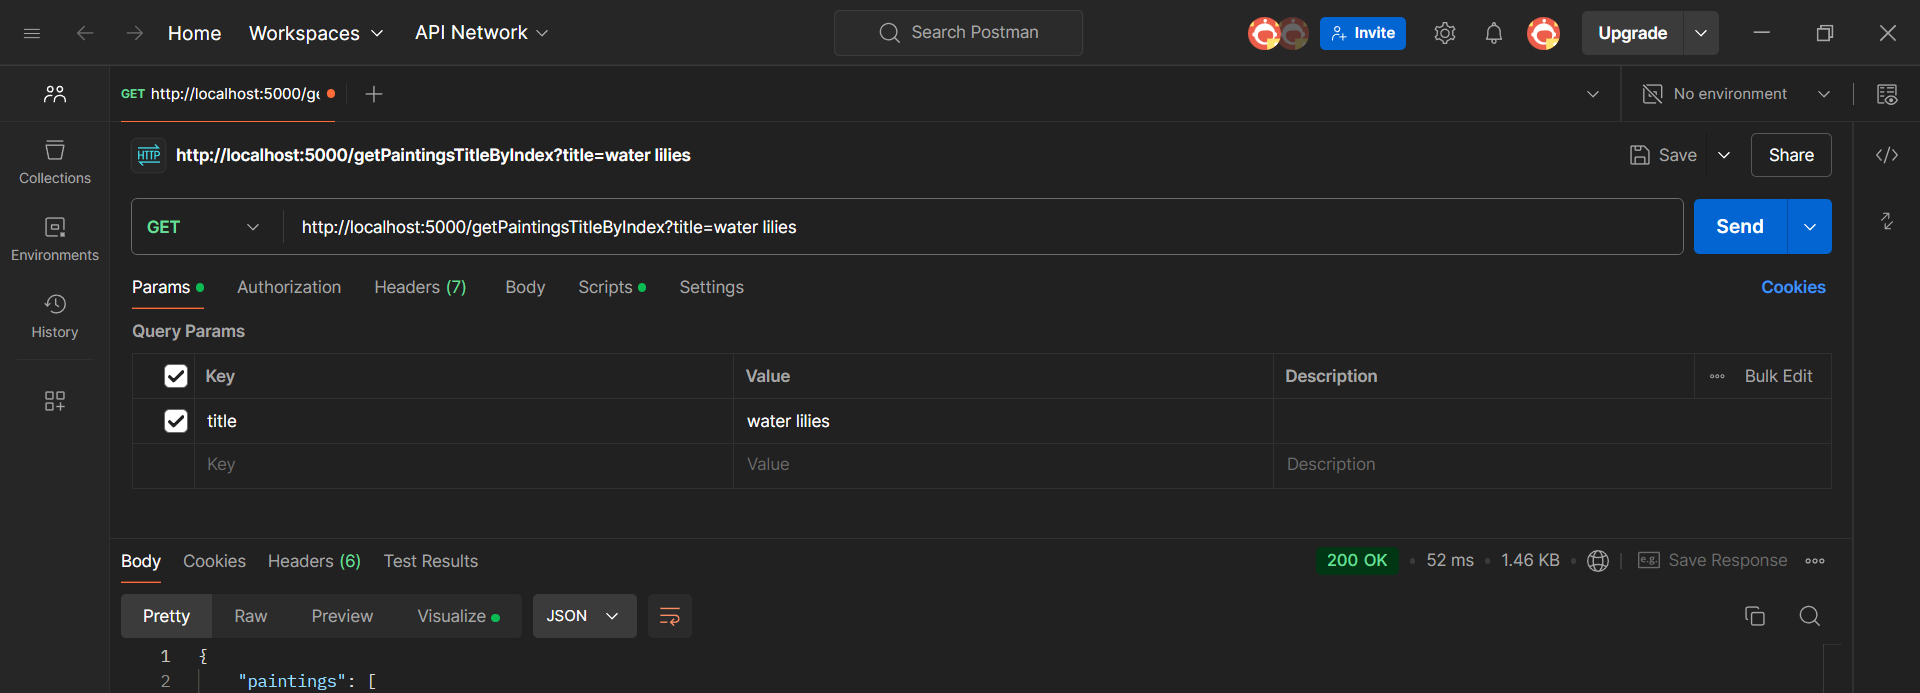
\includegraphics[width=1\textwidth]{images/getPaintingsTitleByIndexS.png}
      \caption{getPaintingsTitleByIndex}
\end{figure}

\subsection{getPaintingsDep vs getPaintingsDepByIndex and getPaintingsArtist vs getPaintingsArtistByIndex}

The functions \textbf{getPaintingsDep} and \textbf{getPaintingsArtist} perform similar operations as the previous ones, but they also create indexing on the departments field and on the artist field. This results in a notable increase in processing speed.

\subsection{getPaintingsFilter vs getPaintingsTitleByIndex}
\textbf{getPaintingsFilter}: The proposed endpoint utilizes a \textbf{compound index} on three fields: \textbf{title, department,} and \textbf{name}.
\begin{lstlisting}[language=Python]
paintings_coll.create_index([("title", ASCENDING), ("department", ASCENDING), ("name", ASCENDING)], name="triple_index")
\end{lstlisting}
The \textbf{triple-index approach} guarantees that the query can rapidly narrow down results based on multiple criteria, making it ideal for \textbf{complex search filters}. The query is constructed as follows:
\begin{lstlisting}[language=Python]
query = {}
if title:
    query["title"] = {"$regex": title, "$options": "i"}
if department:
    query["department"] = {"$regex": department, "$options": "i"}
if name:
    query["name"] = {"$regex": name, "$options": "i"}
\end{lstlisting}
This approach reduces query time by minimizing the need for a full collection scan, even when using \textbf{multiple search parameters}. From a user experience perspective, the ability to search using a compound index allows for greater \textbf{flexibility} and \textbf{time efficiency}, as users can input more search criteria. However, it is important to note that indexing on three fields can negatively impact performance compared to the \textbf{getPaintingsTitleByIndex} function, which uses a single field index.

\subsection{getPaintingsArtistByIndex vs getPaintingsArtistCollection}
\textbf{getPaintingsArtistByIndex}: The function is designed to simplify the retrieval of all paintings created by a specific artist. This is achieved through the use of a search parameter (\textbf{name}), which \textbf{indexes} the \textbf{artist's name} and enables the filtering of data. It optimizes the search process by reducing the number of scanned documents.
\begin{lstlisting}[language=Python]
paintings_coll.create_index([("name", ASCENDING)], name="name_index")
query = {"name": {"$regex": name, "$options": "i"}}
\end{lstlisting}

\textbf{getPaintingsArtistCollection}: On the other hand, this approach dynamically accesses a collection whose name matches the name of the selected artist. Each artist has their own collection containing documents that represent their paintings, created during the data upload phase. Moreover, this structure allows \textbf{flexibility} (each artist can have their own collection schema) but complicates the management of the database.
\begin{lstlisting}[language=Python]
collection = db[name]
paintings = list(collection.find({}))
\end{lstlisting}

\subsection{Conclusion}

Once an index has been created in MongoDB, the resulting index will be of the \textbf{B+-tree variety},which is characterised by frequent read and write activity, which is characterised by frequent read and write activity.
Given the high volume of queries applied to specific elements of the dataset, the use of indexes was identified as an effective method to enhance performance.

\end{document}
